\section{Reactive IPS Modelling} \label{sec:c3_model}

To facilitate the understanding and exploration of reactive IPSs, we present a model which outputs the normalised forward progress \nm{\alpha}{exe}.
Parameters of this model are listed in \tref{tab:parameter}. 
The model assumes that all configuration parameters remain constant. 
We assume that all input and configuration parameters remain constant in this model derivation, but later provide a dynamic process for cases where parameters change dynamically. 

\begin{table}[!t]
    \renewcommand{\arraystretch}{1.2}
    \centering
    \caption{Model parameters of reactive IPS} 
    \label{tab:parameter}
    \begin{tabular}{|c|c|}
        % \hline
        % \textbf{Parameter} & \textbf{Description} \\
        \hline
        \multicolumn{2}{|c|}{\textbf{Input Parameters}}\\
        \hline
        \nm{I}{harv} & Energy harvester current supply\\
        \N{C}& Energy storage capacitance\\
        \hline
        \multicolumn{2}{|c|}{\textbf{Configuration Parameters}}\\
        \hline
        \nm{I}{exe} & Execution current draw\\
        \nm{I}{lpm} & Low-power mode current draw\\
        \nm{I}{r} & Restore current draw\\
        \nm{I}{s} & Save current draw\\
        \nm{I}{leak} & Leakage current draw\\
        \nm{V}{r} & Restore voltage threshold\\
        \nm{V}{s} & Save voltage threshold\\
        \nm{T}{r} & Restore time overhead\\
        \nm{T}{s} & Save time overhead\\
        \hline
        \multicolumn{2}{|c|}{\textbf{Output Parameter}}\\
        \hline
        \nm{\alpha}{exe} & Normalised forward progress \\ 
        \hline
    \end{tabular}
\end{table}

% Since supply current \nm{I}{harv} and leakage current \nm{I}{leak} constantly exist (though could be zero), 
For brevity, \nm{I}{in} denotes the usable input current as expressed in \eref{eq:in}. 
The effect of capacitor leakage current, \nm{I}{leak}, is discussed at the end of \sref{subsec:formulation}.
\begin{equation}
    \nmm{I}{in} = \nmm{I}{harv} - \nmm{I}{leak}
    \label{eq:in}
\end{equation}

\subsection{Operating Modes of Reactive IPS}

The behaviour of reactive IPSs can be classified into three operating modes depending on the supply current, as shown in \fref{fig:operatingModes}. 
These are differentiated by the relationship between input current \nm{I}{in} and the system's current draw in its low-power mode (LPM) or active modes, i.e. \nm{I}{lpm} and \nm{I}{exe}. 
We define the three modes as:

\begin{figure}
    \centering
    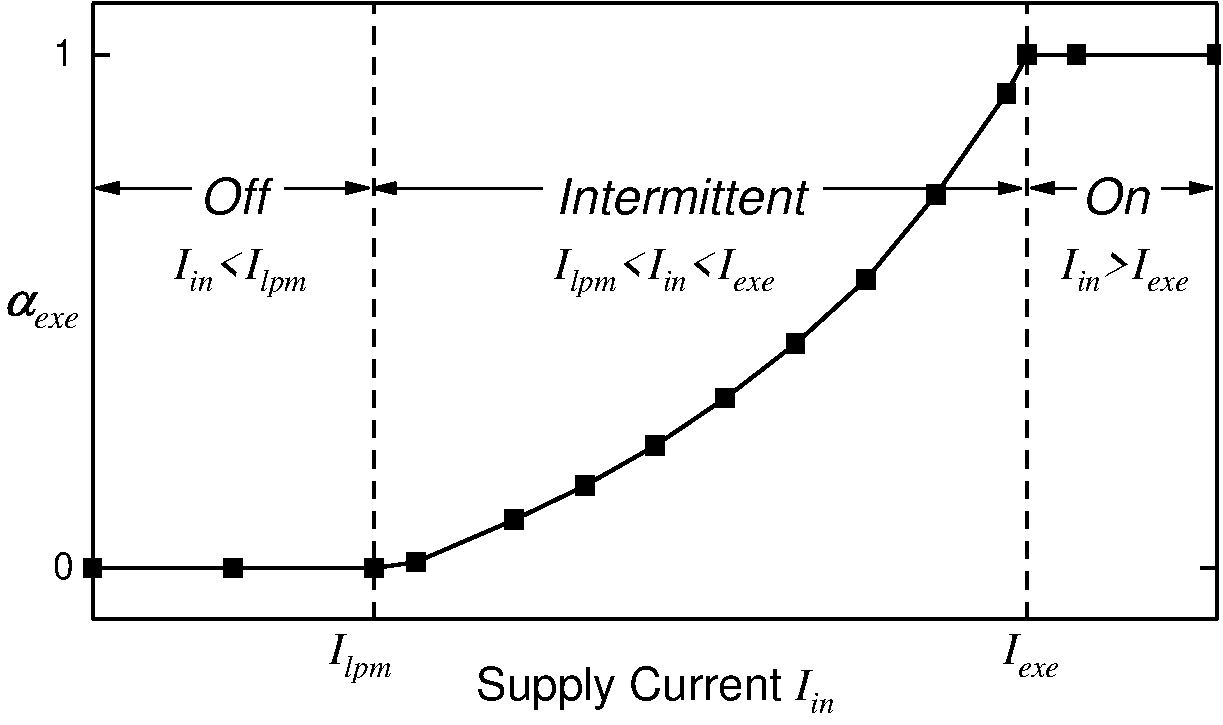
\includegraphics[width=\columnwidth]{ch3_sizingeffect/figures/OperatingMode0Fig}
    \caption{Operating modes of reactive IPSs, and achieved forward progress against supply current.}
    \label{fig:operatingModes}
\end{figure}

\begin{itemize}
	\item \textit{Off} mode: When $\nmm{I}{in} < \nmm{I}{lpm}$, the system stays inactive. 
    The supply voltage \nm{V}{cc} cannot rise above the restore threshold \nm{V}{r} to wake the system and start execution. 
    The LPM current \nm{I}{lpm} includes the consumption of voltage monitoring circuits and system idle current.
	% Here, \nm{I}{lpm} is induced after \nm{V}{cc} goes above the minimum operating voltage $V_{off}$ where the system waits for \nm{V}{cc} to reach \nm{V}{r} (when $V_{off} < \nmm{V}{cc} < \nmm{V}{r}$). 

    \item \textit{On} mode: When $\nmm{I}{in} > \nmm{I}{exe}$, the system executes constantly as the supply voltage \nm{V}{cc} never drops below \nm{V}{s}. 
    \nm{V}{cc} grows until \nm{I}{in} and \nm{I}{exe} are in equilibrium, which may result from \nm{I}{in} decreasing due to poor impedance matching, or \nm{I}{exe} increasing due to either greater current draw at higher voltage or dissipation through overvoltage protection circuits. 

	\item \textit{Intermittent} mode: When $\nmm{I}{lpm} < \nmm{I}{in} < \nmm{I}{exe}$, the system executes intermittently after $\nmm{V}{cc} > \nmm{V}{r}$ and before $\nmm{V}{cc} < \nmm{V}{s}$. \nm{V}{cc} can rise above \nm{V}{r} and the system starts execution. 
	However, the stored energy is then consumed by the load as $\nmm{I}{in} < \nmm{I}{exe}$, causing \nm{V}{cc} to eventually drop below the save threshold \nm{V}{s}, where the system saves its state and enters LPM. 
	The system stays in LPM until \nm{V}{cc} rises to \nm{V}{r} again and then resumes execution. 
	% In this mode, \nm{V}{cc} oscillates approximately between \nm{V}{r} and \nm{V}{s}, 'switching' on and off the execution. 
    In general, a higher \nm{I}{in} leads to more forward progress in this mode, but the exact relationship between \nm{I}{in} and forward progress requires further analysis.
    
	% The excess power either dissipates through circuits or overcharges \nm{V}{cc}. An overcharged \nm{V}{cc} may affect harvesting efficiency due to poor impedance matching and reduce \nm{I}{harv}, such that current input and consumption are in equilibrium. 
	% In this model case, charging \nm{V}{cc} above the maximum power point of the PV cell reduces $I_{harvest}$, and \nm{V}{cc} is stable when $I_{harvest} = \nmm{I}{exe} + \nmm{I}{leak}$. 
\end{itemize}

\subsection{Formulating Forward Progress} \label{subsec:formulation}

Next, we derive formulations to calculate \nm{\alpha}{exe} from \nm{I}{in} and energy storage capacitance \N{C}. 
We then explore the effect of capacitor leakage on maximum forward progress. 

In the \textit{On} and \textit{Off} modes, the normalised forward progress is trivial to find (simply 1 and 0 respectively). 
In the \textit{Intermittent} mode,  as shown in \fref{fig:operatingCycle}, the system goes through four intervals in turn, i.e. charging, restoring, executing, and saving, with current consumption of \nm{I}{lpm}, \nm{I}{r}, \nm{I}{exe}, and \nm{I}{s} in each interval respectively. 
The normalised forward progress, i.e. effective execution time ratio, is indicated as $\nmm{T}{exe} / \nmm{T}{cycle}$, where \nm{T}{exe} is the time spent on effective execution in one operating cycle and \nm{T}{cycle} is the period of operating cycles. 
Hence, the forward progress given all supply levels is expressed as:
\begin{equation}
    \nmm{\alpha}{exe} = \left\{
    \begin{aligned}
        & 0 & , & \quad \textit{Off} \, (\nmm{I}{in} < \nmm{I}{lpm}) \\
        & \frac{\nmm{T}{exe}}{\nmm{T}{cycle}} & , & \quad \textit{Intermittent} \, (\nmm{I}{lpm} < \nmm{I}{in} < \nmm{I}{exe}) \\
        & 1 & , & \quad \textit{On} \, (\nmm{I}{in} > \nmm{I}{exe})
    \end{aligned}
    \right.
    \label{eq:feff}
\end{equation}

\begin{figure}
    \centering
    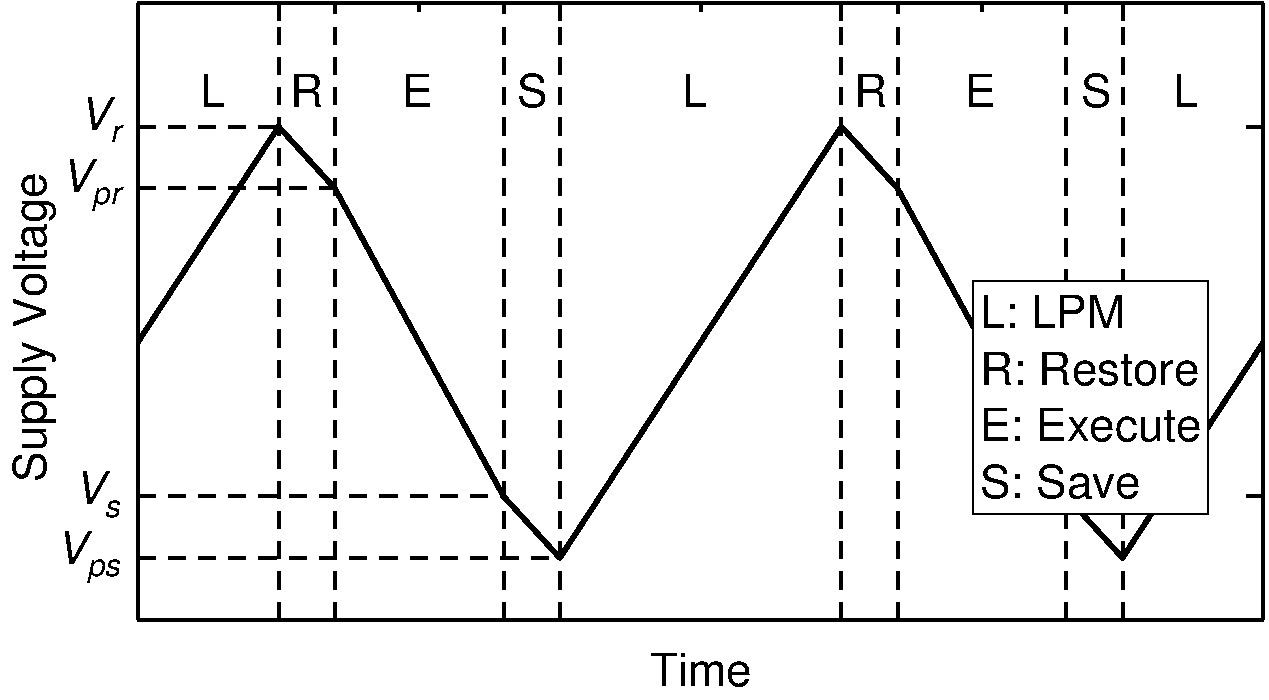
\includegraphics[width=\columnwidth]{ch3_sizingeffect/figures/CRESdemoFig}
    \caption{Operating cycles in the \textit{Intermittent} mode. }
    \label{fig:operatingCycle}
\end{figure}

In the following analysis, we focus on deriving $\nmm{T}{exe} / \nmm{T}{cycle}$ in the \textit{Intermittent} mode. 
Let \nm{V}{pr} (post-restore) and \nm{V}{ps} (post-save) denote the voltage after restoring and saving operations. 
Referring to \tref{tab:parameter} and \fref{fig:operatingCycle}, \nm{V}{pr} and \nm{V}{ps} can be calculated as:
\begin{equation}
    \nmm{V}{pr} = \nmm{V}{r} + \frac{\nmm{T}{r} (\nmm{I}{in} - \nmm{I}{r})}{C}
    \label{eq:vpr}
\end{equation}
\begin{equation}
    \nmm{V}{ps} = \nmm{V}{s} + \frac{\nmm{T}{s} (\nmm{I}{in} - \nmm{I}{s})}{C}
    \label{eq:vps}
\end{equation}
With \eref{eq:vpr}, the time spent on effective execution \nm{T}{exe} in one operating cycle can be expressed as:
\begin{equation}
    \begin{aligned}
        \nmm{T}{exe} & = \frac{C(\nmm{V}{pr} - \nmm{V}{s})}{\nmm{I}{exe} - \nmm{I}{in}} \\
        & = \frac{C(\nmm{V}{r} - \nmm{V}{s}) + \nmm{T}{r} (\nmm{I}{in} - \nmm{I}{r})} {\nmm{I}{exe} - \nmm{I}{in}}
    \end{aligned}
    \label{eq:texe}
\end{equation}
Analogously, with \eref{eq:vps}, the charging interval can be described as:
\begin{equation}
    \begin{aligned}
        T_{charge} & = \frac{C(\nmm{V}{r} - \nmm{V}{ps})}{\nmm{I}{in} - \nmm{I}{lpm}} \\
        & = \frac{C(\nmm{V}{r} - \nmm{V}{s}) - \nmm{T}{s} (\nmm{I}{in} - \nmm{I}{s})} {\nmm{I}{in} - \nmm{I}{lpm}}
    \end{aligned}
    \label{eq:tcharge}
\end{equation}
With \eref{eq:texe} and \eref{eq:tcharge}, the period of an operating cycle is:
\begin{equation}
    \begin{aligned}
        \nmm{T}{cycle} & = T_{charge} + \nmm{T}{r} + \nmm{T}{exe} + \nmm{T}{s} \\
        & = \frac{C (\nmm{V}{r} - \nmm{V}{s}) + \nmm{T}{s} (\nmm{I}{s} - \nmm{I}{lpm})}{\nmm{I}{in} - \nmm{I}{lpm}} + \frac{C (\nmm{V}{r} - \nmm{V}{s}) + \nmm{T}{r} (\nmm{I}{exe} - \nmm{I}{r})}{\nmm{I}{exe} - \nmm{I}{in}}
    \end{aligned}
    \label{eq:tperiod}
\end{equation}

Finally, combining \eref{eq:vpr} to \eref{eq:tperiod}, we obtain normalised forward progress \nm{\alpha}{exe} in the \textit{Intermittent} mode ($\nmm{I}{lpm} < \nmm{I}{in} < \nmm{I}{exe}$) as:
\begin{equation}
    \begin{aligned}
        \nmm{\alpha}{exe} &= \frac{\nmm{T}{exe}}{\nmm{T}{cycle}} \\
        &= [\frac{C (\nmm{V}{r} - \nmm{V}{s}) + \nmm{T}{r} (\nmm{I}{in} - \nmm{I}{r})} {\nmm{I}{exe} - \nmm{I}{in}}] / \\
        &[\frac{C (\nmm{V}{r} - \nmm{V}{s}) + \nmm{T}{s} (\nmm{I}{s} - \nmm{I}{lpm})}{\nmm{I}{in} - \nmm{I}{lpm}} + \frac{C (\nmm{V}{r} - \nmm{V}{s}) + \nmm{T}{r} (\nmm{I}{exe} - \nmm{I}{r})}{\nmm{I}{exe} - \nmm{I}{in}}] \\
    \end{aligned}
    \label{eq:texepercent}
\end{equation}
In the numerator \nm{T}{exe}, $C(\nmm{V}{r} - \nmm{V}{s})$ represents the amount of charge in the capacitor available for restoring and executing. 
$\nmm{T}{r} (\nmm{I}{in} - \nmm{I}{r})$ represents the charge used by a restore operation. 
$\nmm{I}{exe} - \nmm{I}{in}$ is the rate of charge consumption from the energy storage during execution.

Also, the ratio of the time overhead on state-saving and -restoring operations to the total elapsed time \nm{T}{rs\%} can be deduced as:
\begin{equation}
    \begin{aligned}
        \nmm{T}{rs\%} &= \frac{\nmm{T}{r} + \nmm{T}{s}}{\nmm{T}{cycle}} \\
        &= (\nmm{T}{r} + \nmm{T}{s}) / [\frac{C (\nmm{V}{r} - \nmm{V}{s}) + \nmm{T}{s} (\nmm{I}{s} - \nmm{I}{lpm})}{\nmm{I}{in} - \nmm{I}{lpm}} + \frac{C (\nmm{V}{r} - \nmm{V}{s}) + \nmm{T}{r} (\nmm{I}{exe} - \nmm{I}{r})}{\nmm{I}{exe} - \nmm{I}{in}}]
    \end{aligned}
    \label{eq:trs}
\end{equation}
\eref{eq:trs} can describe the impact of state-saving and -restoring overhead with respect to \N{C} and \nm{I}{in}.

% \footnote{Calculation breakdowns of differential analysis is attached in Appendix.}
% Higher \nm{\alpha}{exe} leads to more time spent on forward progress. 
% As $d\nmm{\alpha}{exe} / d\nmm{I}{in}$ is positive, higher harvested current \nm{I}{harv} leads to more forward progress. 

To explore the effect of energy storage on forward progress, we need to analyse $d\nmm{\alpha}{exe} / dC$. 
Here, if we assume that \nm{I}{leak} remains constant, \nm{\alpha}{exe} keeps increasing and approaches $(\nmm{I}{in} - \nmm{I}{lpm}) / (\nmm{I}{exe} - \nmm{I}{lpm})$ when energy storage capacitance \N{C} increases. 
Defining $(\nmm{I}{in} - \nmm{I}{lpm}) / (\nmm{I}{exe} - \nmm{I}{lpm})$ as \nm{\alpha}{exe\_ideal}, $\nmm{\alpha}{exe} = \nmm{\alpha}{exe\_ideal}$ is an ideal case, where state-saving and -restoring overheads are absent.

In an electrolytic capacitor, however, \nm{I}{leak} typically increases with \N{C} with the following relationship~\cite{avxleakage}:
% \cite{alcapacitor}
\begin{equation}
    \nmm{I}{leak} = kC\nmm{V}{cc}
    \label{eq:ileak}
\end{equation}
where $k$ is a constant normally in a range of \SIrange{0.01}{0.03}{\ampere\per\farad\per\volt}. 
Combining \eref{eq:ileak} with \eref{eq:in}, $d\nmm{I}{in} / dC$ is $-k\nmm{V}{cc}$, meaning \nm{I}{in} decreases linearly as \N{C} increases. 
Thus, when \N{C} increases, \nm{\alpha}{exe} keeps approaching \nm{\alpha}{exe\_ideal} while \nm{\alpha}{exe\_ideal} decreases. 
Hence, we believe that there is a capacitance value that leads to the maximum \nm{\alpha}{exe} considering \nm{I}{leak} increases with \N{C}.

\subsection{Dynamic process}

The abovex model assumes all parameters are constant, which is useful for fast exploration in cases where this can be considered to approximately hold true (this is used for the analysis of principal sizing effects presented in \sref{sec:c3_exploration}).
For dynamically-varying parameters (e.g. a dynamic harvesting profile), we also implement a dynamic process, where the supply voltage is calculated with system's current flows and energy storage capacitance across small time steps, hence updating system state accurately. 
This is used for the exploration of real-world energy conditions in \sref{section:demo}.
